%% LyX 2.2.3 created this file.  For more info, see http://www.lyx.org/.
%% Do not edit unless you really know what you are doing.
\documentclass[oneside,english]{extbook}
\usepackage[T1]{fontenc}
\usepackage[latin9]{inputenc}
\usepackage[a4paper]{geometry}
\geometry{verbose,tmargin=25mm,bmargin=25mm,lmargin=25mm,rmargin=25mm}
\setcounter{secnumdepth}{3}
\setcounter{tocdepth}{3}
\setlength{\parindent}{0bp}
\synctex=1
\usepackage{color}
\usepackage{babel}
\usepackage{float}
\usepackage{amstext}
\usepackage{graphicx}
\usepackage{setspace}
\onehalfspacing
\usepackage[unicode=true,
 bookmarks=true,bookmarksnumbered=false,bookmarksopen=false,
 breaklinks=false,pdfborder={0 0 1},backref=false,colorlinks=true]
 {hyperref}
\hypersetup{
 pdfauthor={Juan Francisco Rasc�n}}

\makeatletter
%%%%%%%%%%%%%%%%%%%%%%%%%%%%%% User specified LaTeX commands.
\usepackage{amssymb}
\usepackage{color}
\usepackage{listings}
\definecolor{hellgelb}{rgb}{1,1,0.85}
\definecolor{colKeys}{rgb}{0,0,1}
\definecolor{colIdentifier}{rgb}{0,0,0}
\definecolor{colComments}{rgb}{1,0,0}
\definecolor{colString}{rgb}{0,0.5,0}
\lstset{
      language=Matlab,
      float=hbp,
      basicstyle=\footnotesize\ttfamily,
      identifierstyle=\color{colIdentifier},
      keywordstyle=\color{colKeys},
      stringstyle=\color{colString},
      commentstyle=\itshape\color{colComments},
      columns=fixed,
      tabsize=4,
      frame=single,
      framerule=1pt,
      extendedchars=true,
      showspaces=false,
      showstringspaces=false,
      numbers=left,
      numberstyle=\tiny\ttfamily,
      numbersep=1em,
      breaklines=true,
      breakindent=10pt,
      backgroundcolor=\color{hellgelb},
      breakautoindent=true,
      captionpos=t,
      xleftmargin=1em,
      xrightmargin=\fboxsep
}
\usepackage{lscape}
\usepackage{amsmath}
\usepackage{mathtools}
\usepackage{pifont}
\usepackage{color}
\usepackage{pdfpages}
\usepackage{accents}
\delimitershortfall=-1pt
\let\Right\right
\let\Left\left
\makeatletter
\def\right#1{\Right#1\@ifnextchar){\!\right}{}}
\def\left#1{\Left#1\@ifnextchar({\!\left}{}}
\makeatother

\setcounter{MaxMatrixCols}{20}

\makeatother

\begin{document}
\pagenumbering{gobble}

\section*{THE POTENTIAL FIELD AROUND THE OBSTACLES}

\begin{figure}[H]
\centering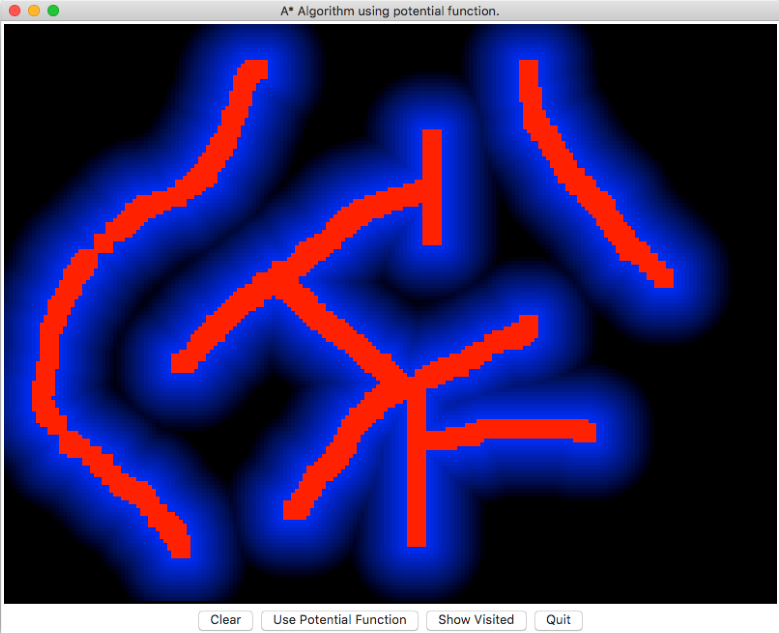
\includegraphics[scale=0.95]{../FIGURES/fig28}
\end{figure}

\newpage

\textbf{Distance transform}\footnote{The previous information was gathered form: https://homepages.inf.ed.ac.uk/rbf/HIPR2/distance.htm}

The distance transform is an operator normally only applied to \textbf{binary
images}(so, binary matrices) . The result of the transform is a \textbf{graylevel
image }of the\textbf{ pixels }that are\textbf{ inside }the\textbf{
foreground regions}. The resulting image looks similar to the input
image. Those graylevel intensities of the pixels that are inside the
foreground regions show the \textbf{distance} to the \textbf{closest
boundary} from each point (\emph{in our case the distance from each
free space node to the closest obstacle node}). \\

One way to think about the distance transform is to first imagine
that foreground regions in the input binary image are made of some
uniform slow burning inflammable material. Then consider simultaneously
starting a fire at all points on the boundary of a foreground region
and letting the fire burn its way into the interior. If we then label
each point in the interior with the amount of time that the fire took
to first reach that point, then we have effectively computed the distance
transform of that region. \\

There are several different sorts of distance transform, depending
upon which distance metric is being used to determine the distance
between pixels. The most common distance metrics are: the \textbf{chessboard}
distance metric, the \textbf{Euclidean} distance metric and the \textbf{city
block} distance metric (aka \textbf{Manhattan} distance metric).

\begin{figure}[H]
\centering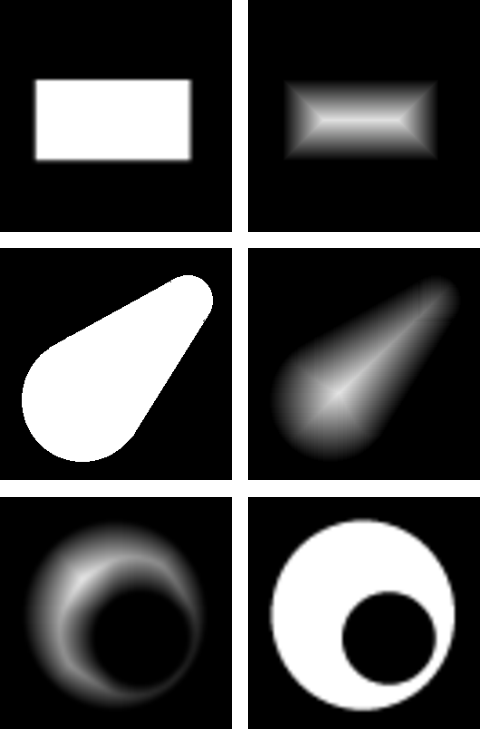
\includegraphics[scale=0.95]{../FIGURES/fig29}

\caption{Euclidean distance transforms}
\end{figure}

There is a dual to the distance transform described above which produces
the distance transform for the background region rather than the foreground
region. It can be considered as a process of inverting the original
image and then applying the standard transform as above.\\

\textbf{How it works}

The distance transform can be calculated efficiently using clever
algorithms in only two passes (e.g. Rosenfeld and Pfaltz 1968). 

In python you should use:
\begin{center}
\texttt{scipy.ndimage.morphology.distance\_transform\_edt(input\_binary\_matrix)}
\par\end{center}

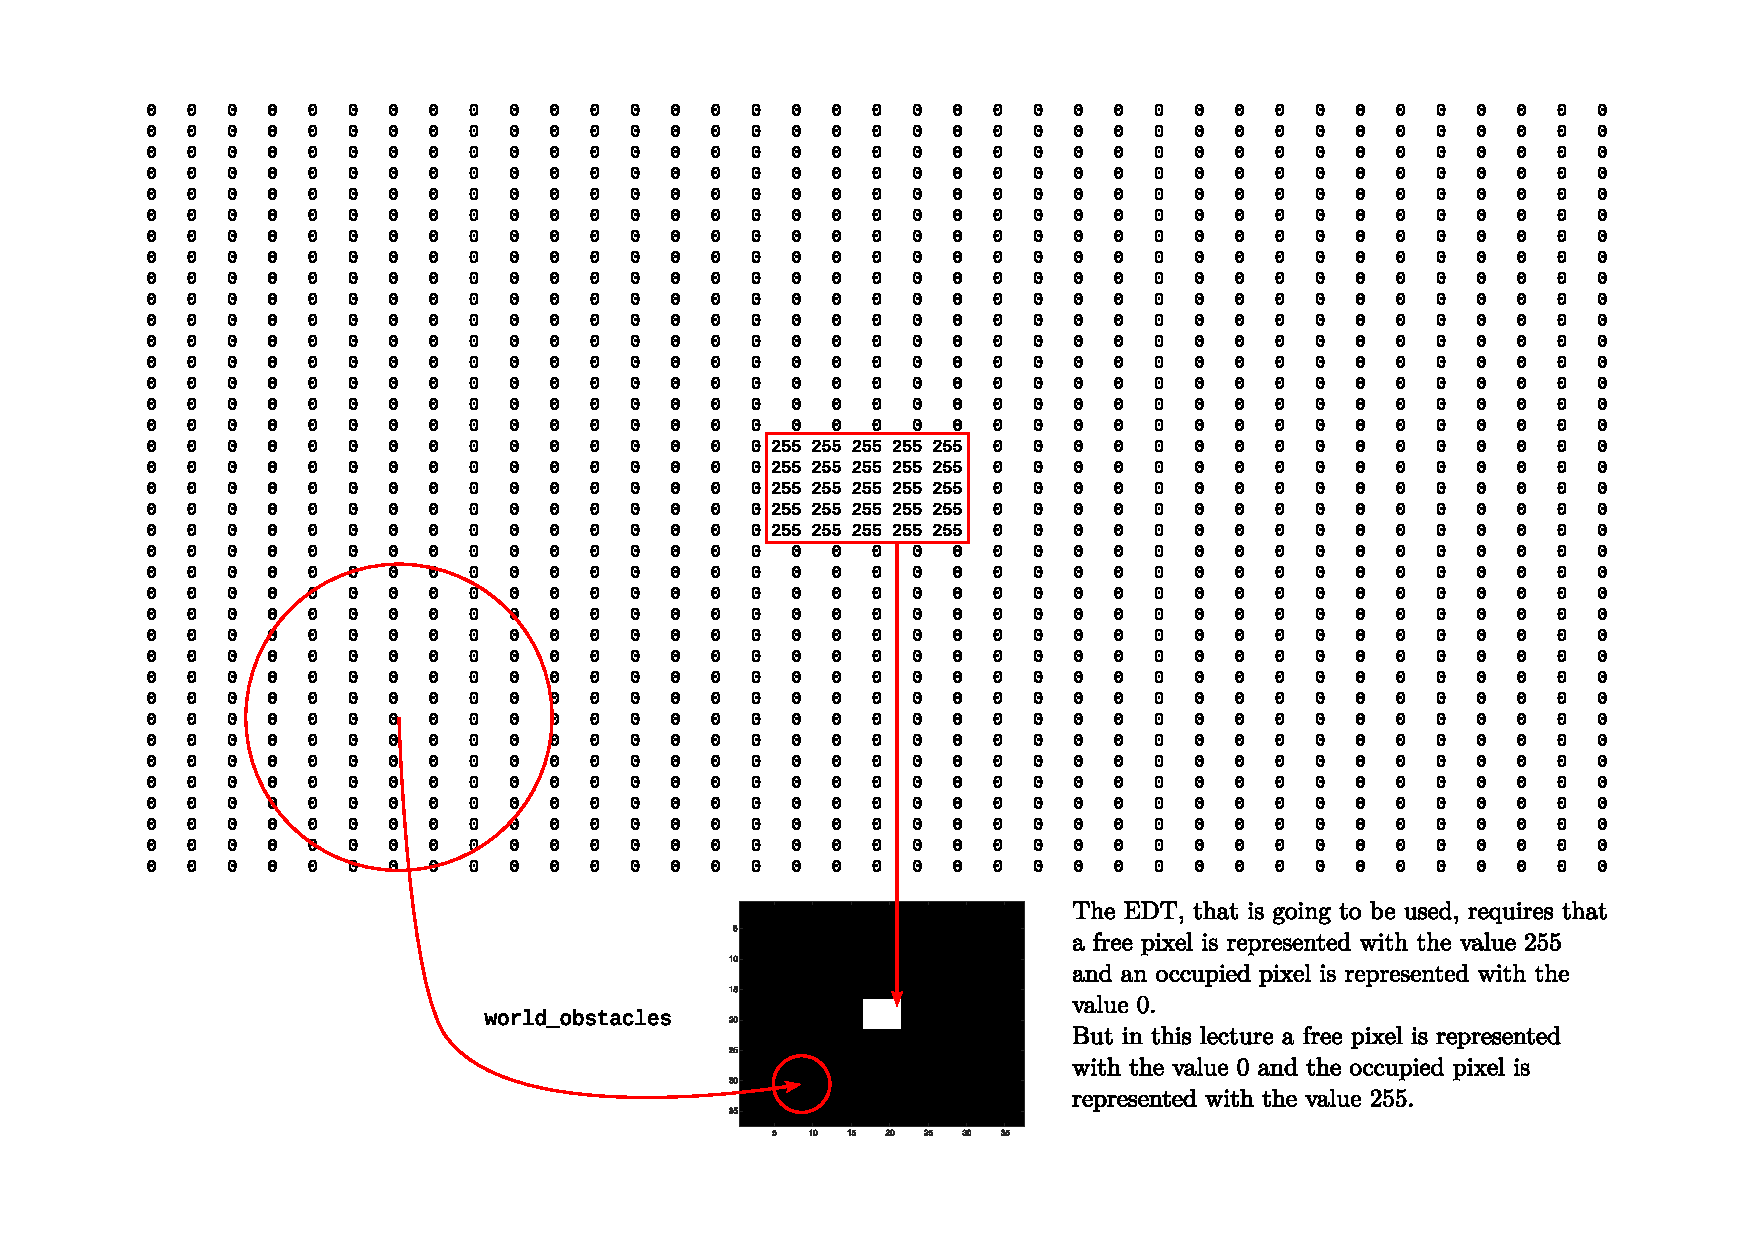
\includepdf[landscape=true]{../FIGURES/fig32.pdf}

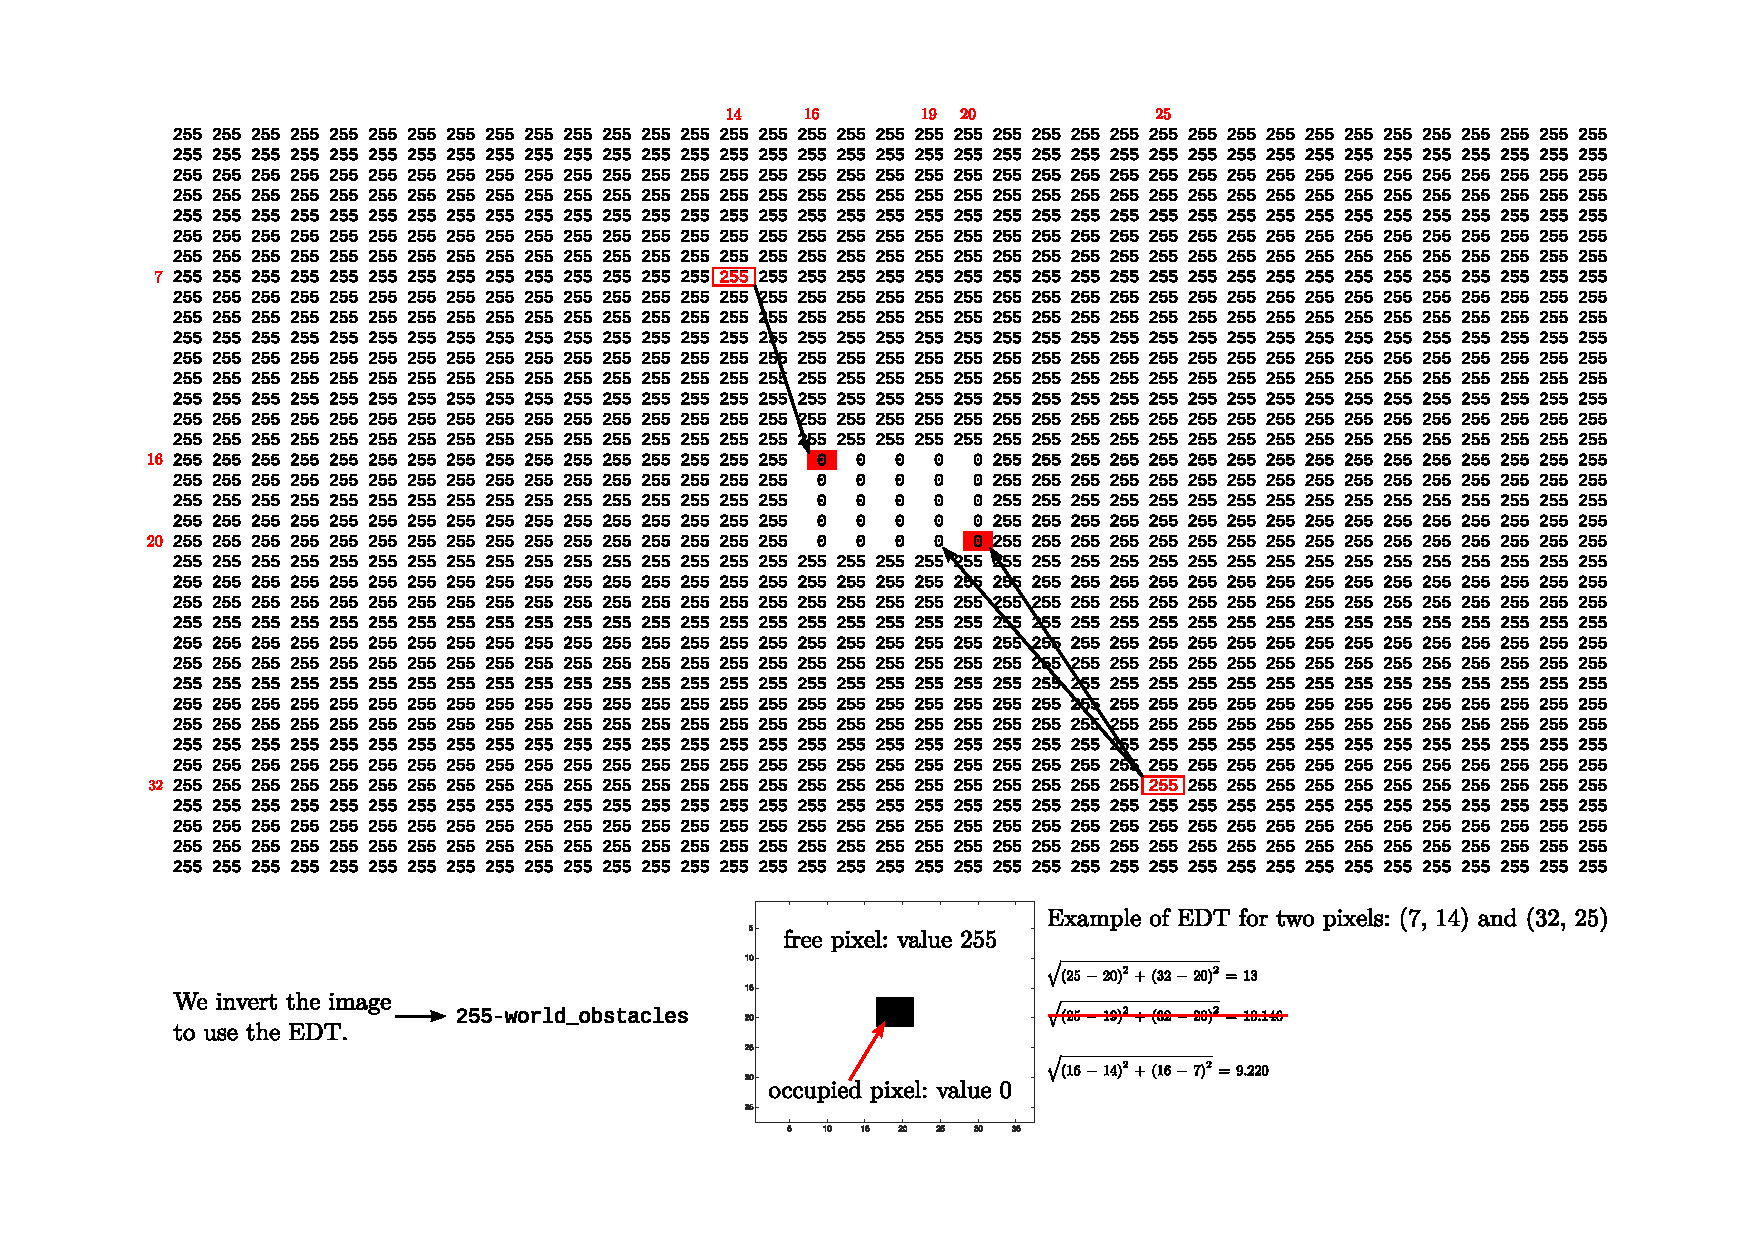
\includepdf[landscape=true]{../FIGURES/fig34.pdf}

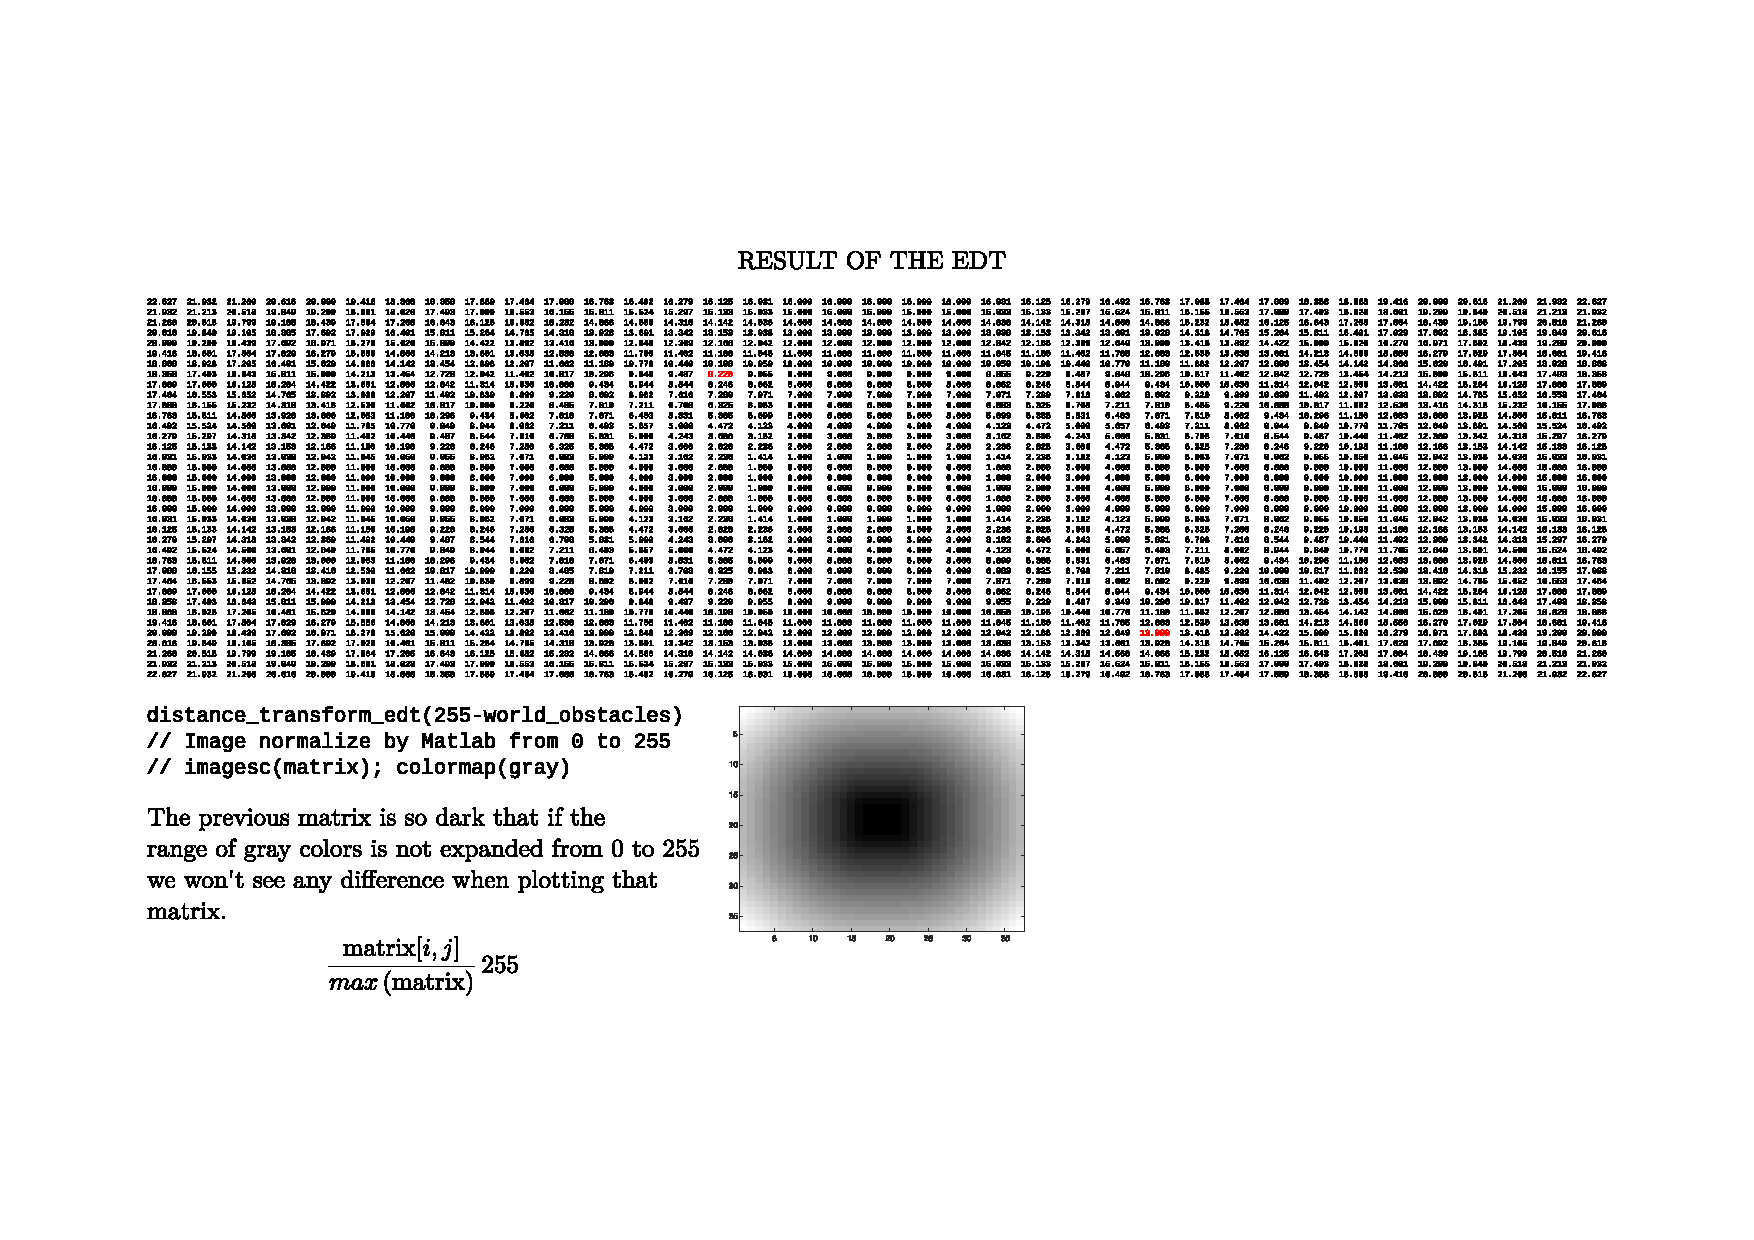
\includepdf[landscape=true]{../FIGURES/fig36.pdf}

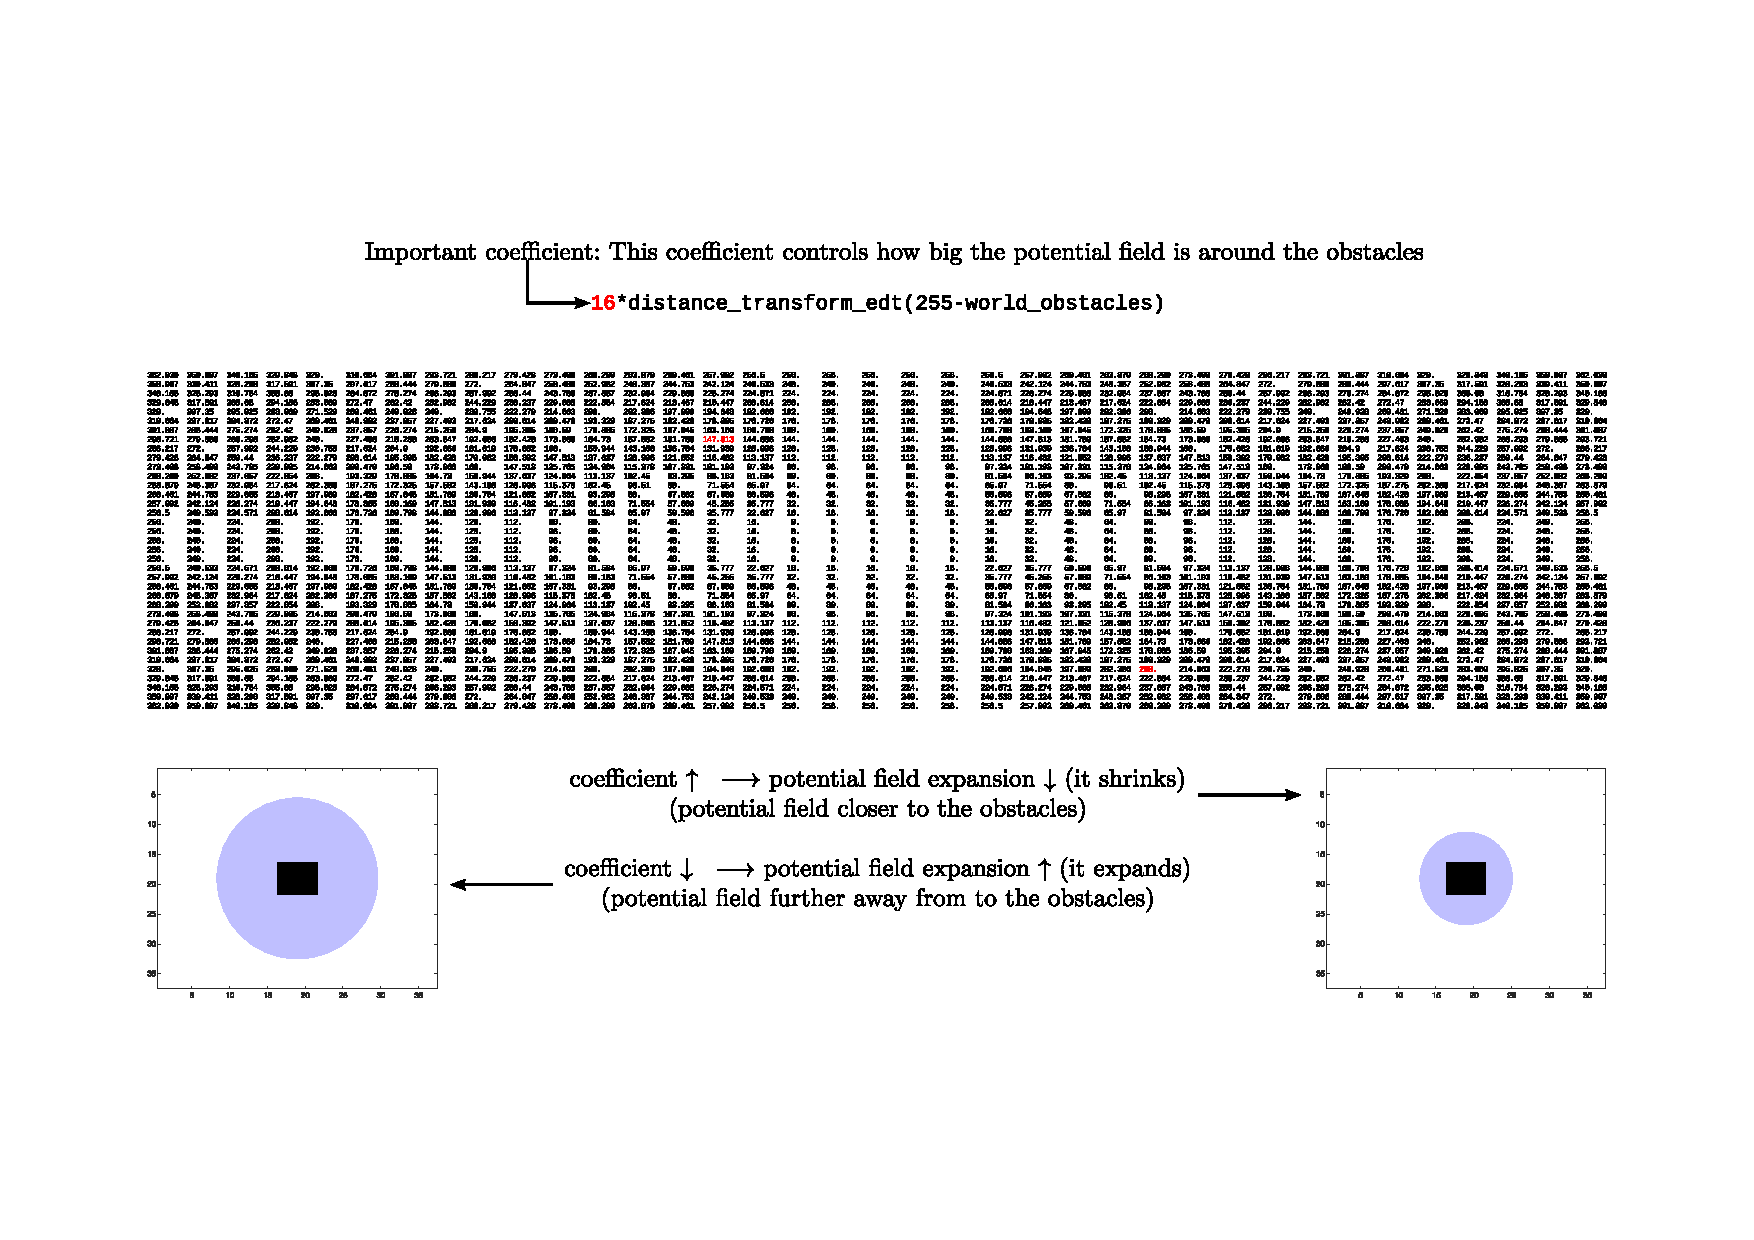
\includepdf[landscape=true]{../FIGURES/fig38.pdf}

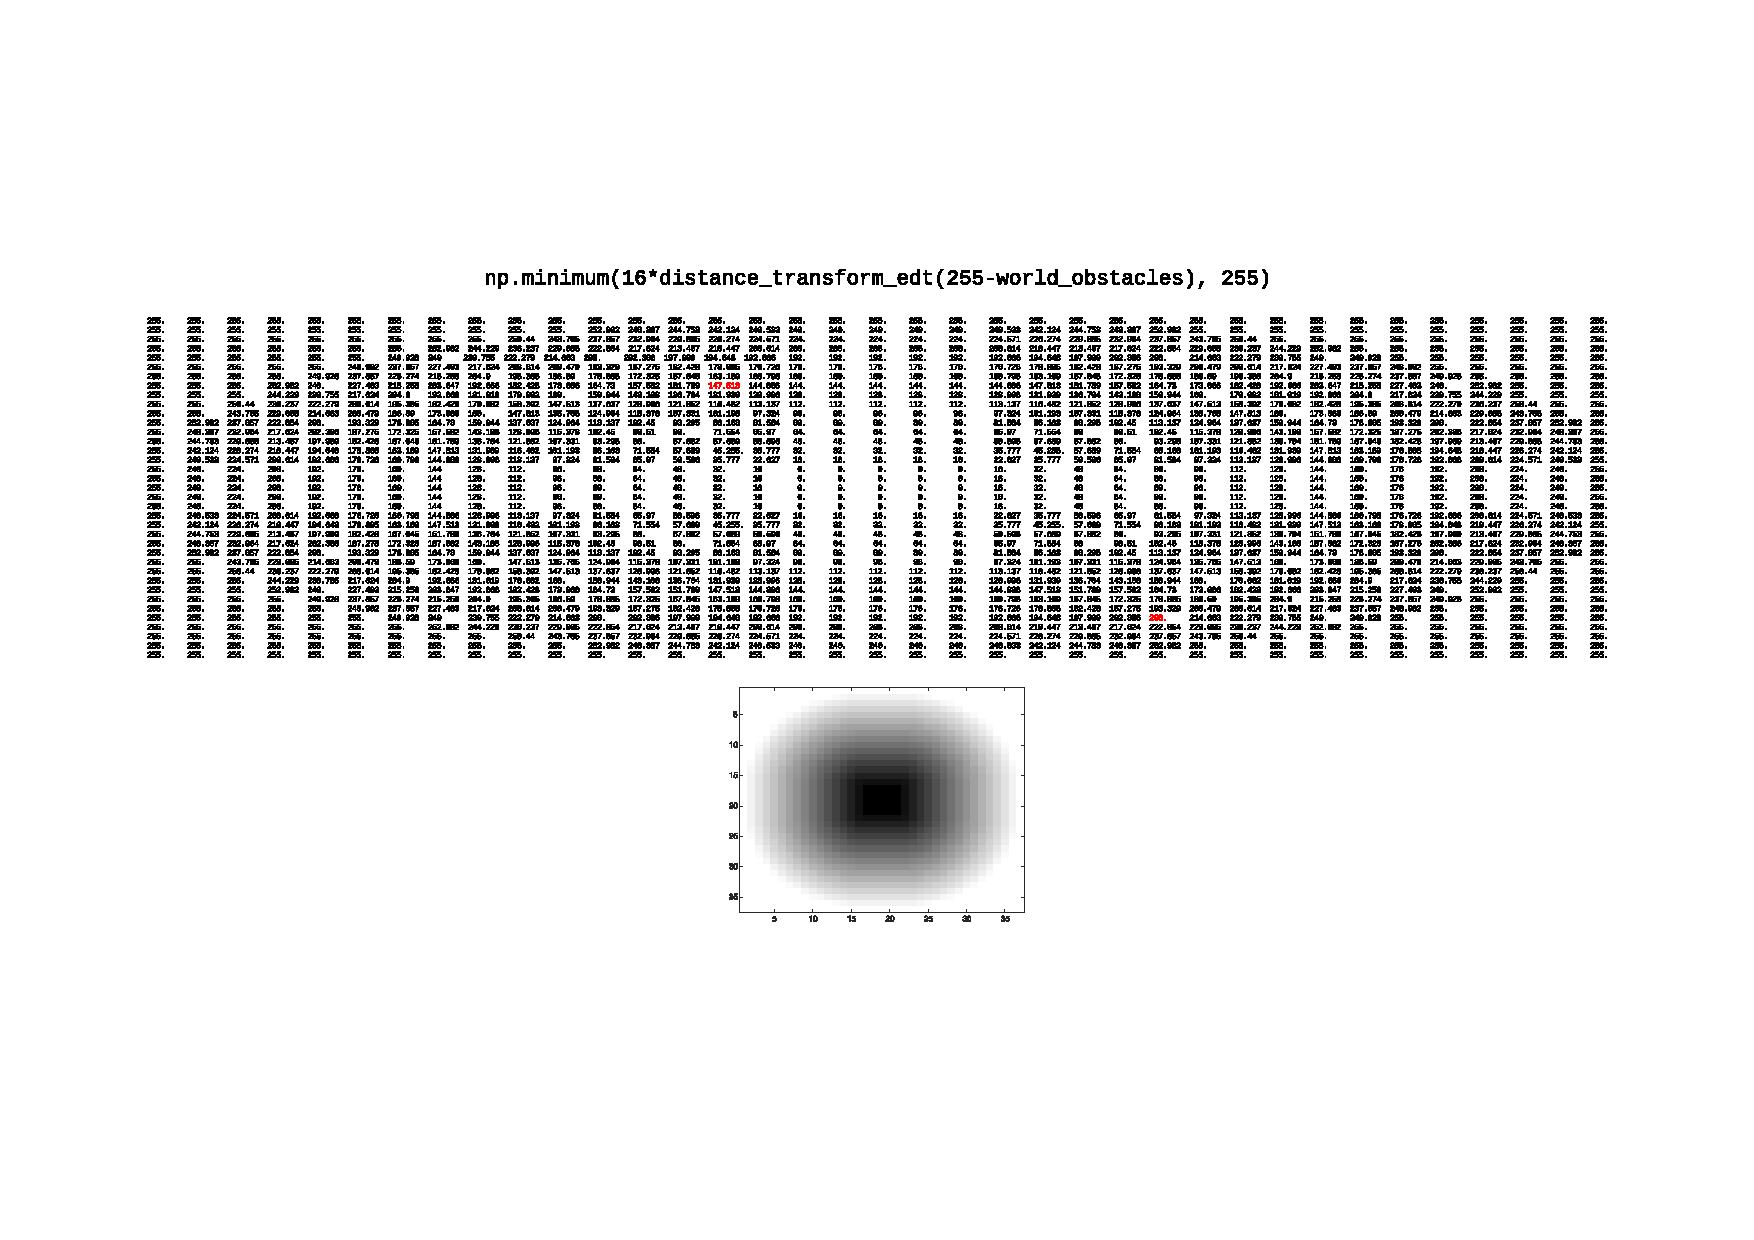
\includepdf[landscape=true]{../FIGURES/fig40.pdf}

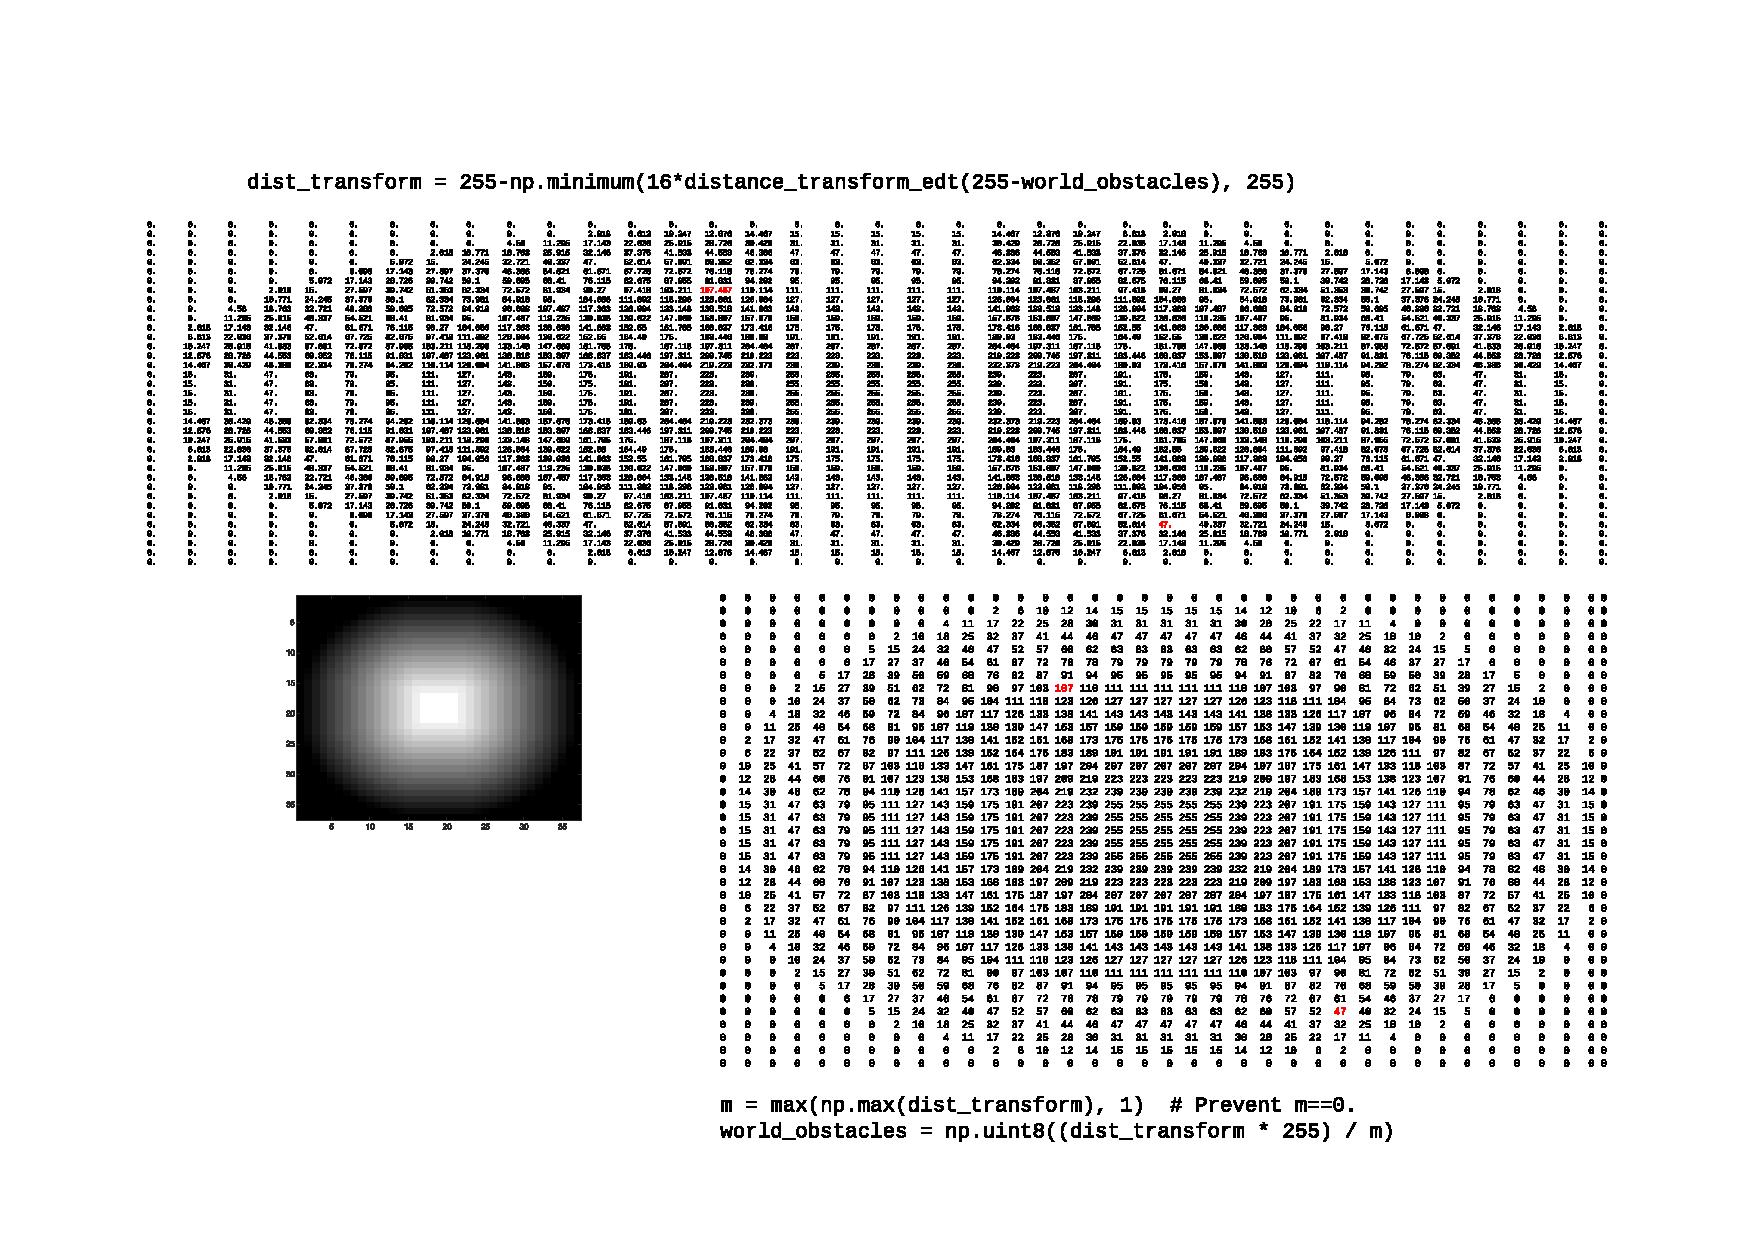
\includepdf[landscape=true]{../FIGURES/fig42.pdf}

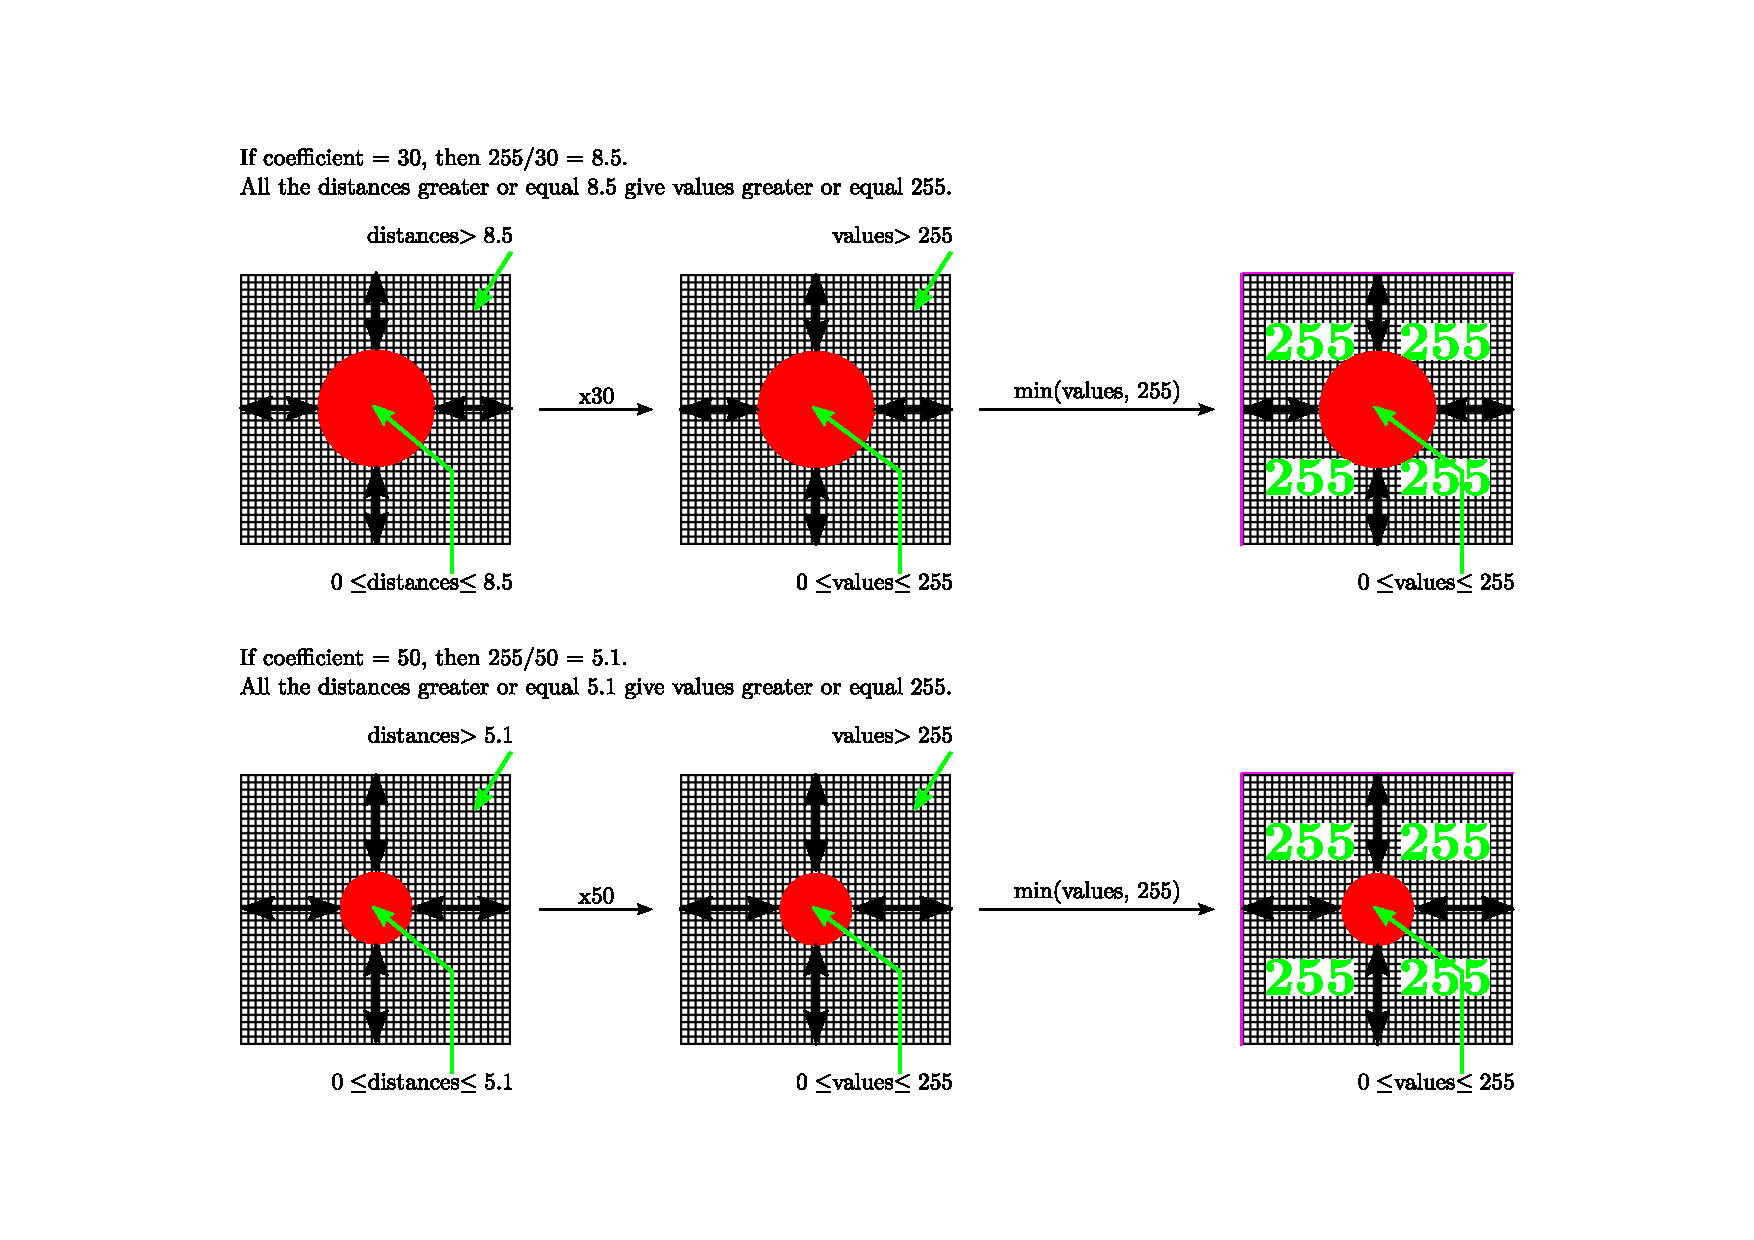
\includepdf[landscape=true]{../FIGURES/fig45.pdf}

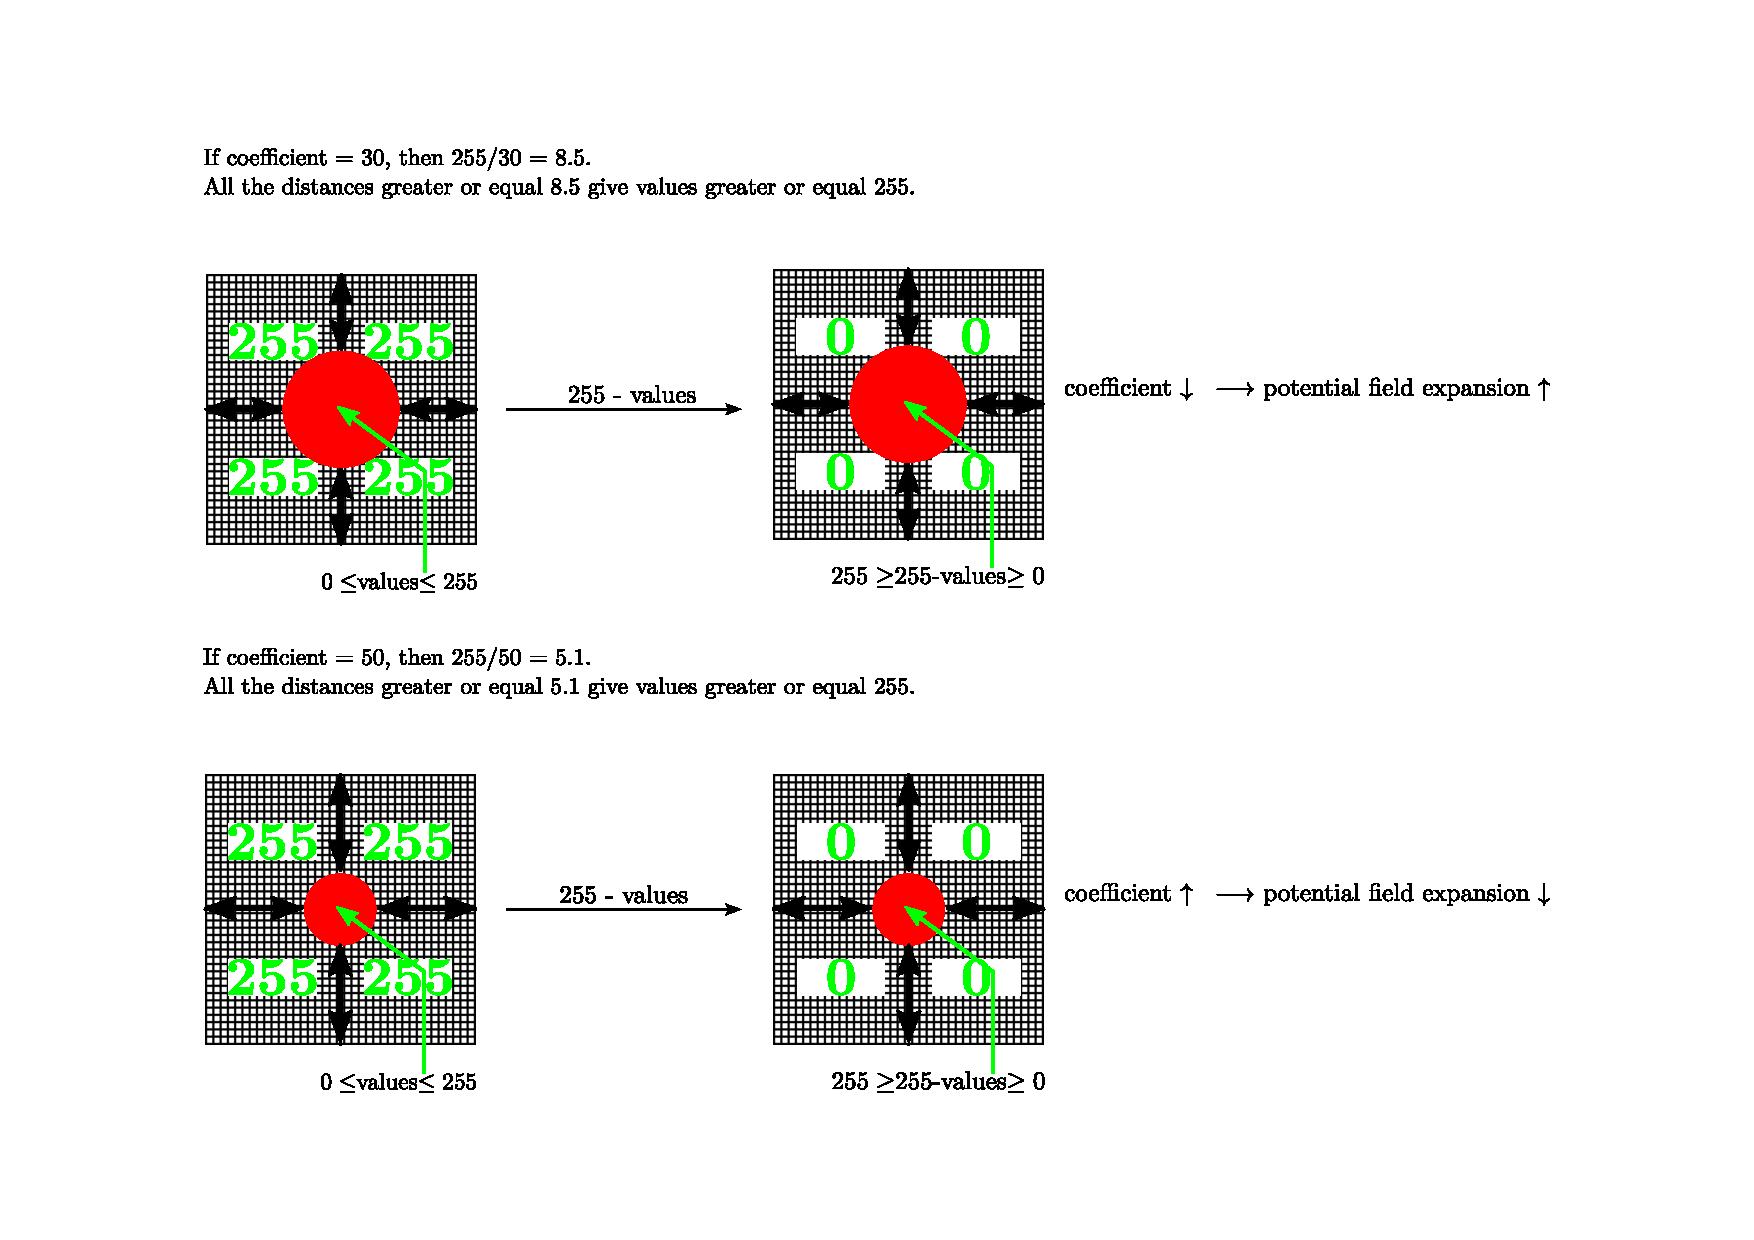
\includepdf[landscape=true]{../FIGURES/fig47.pdf}

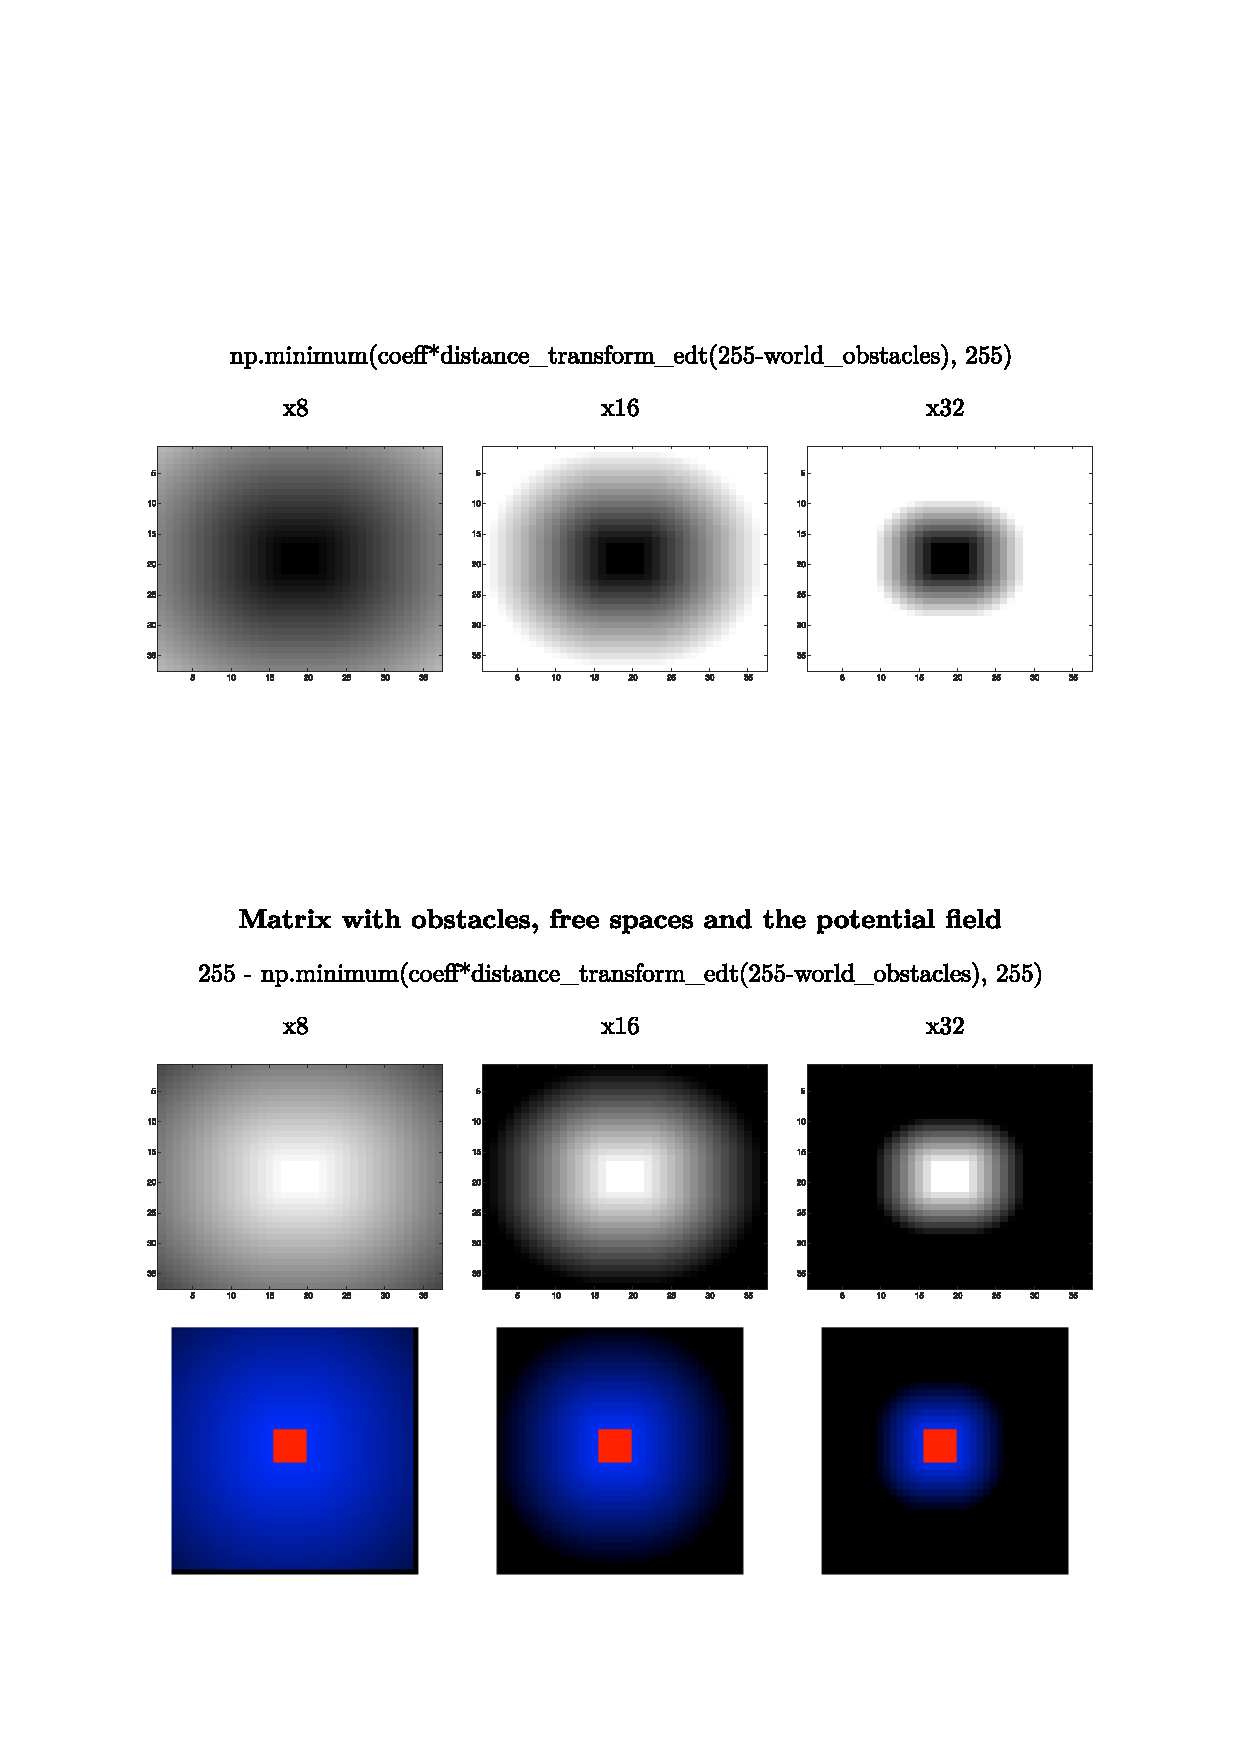
\includepdf{../FIGURES/fig50.pdf}

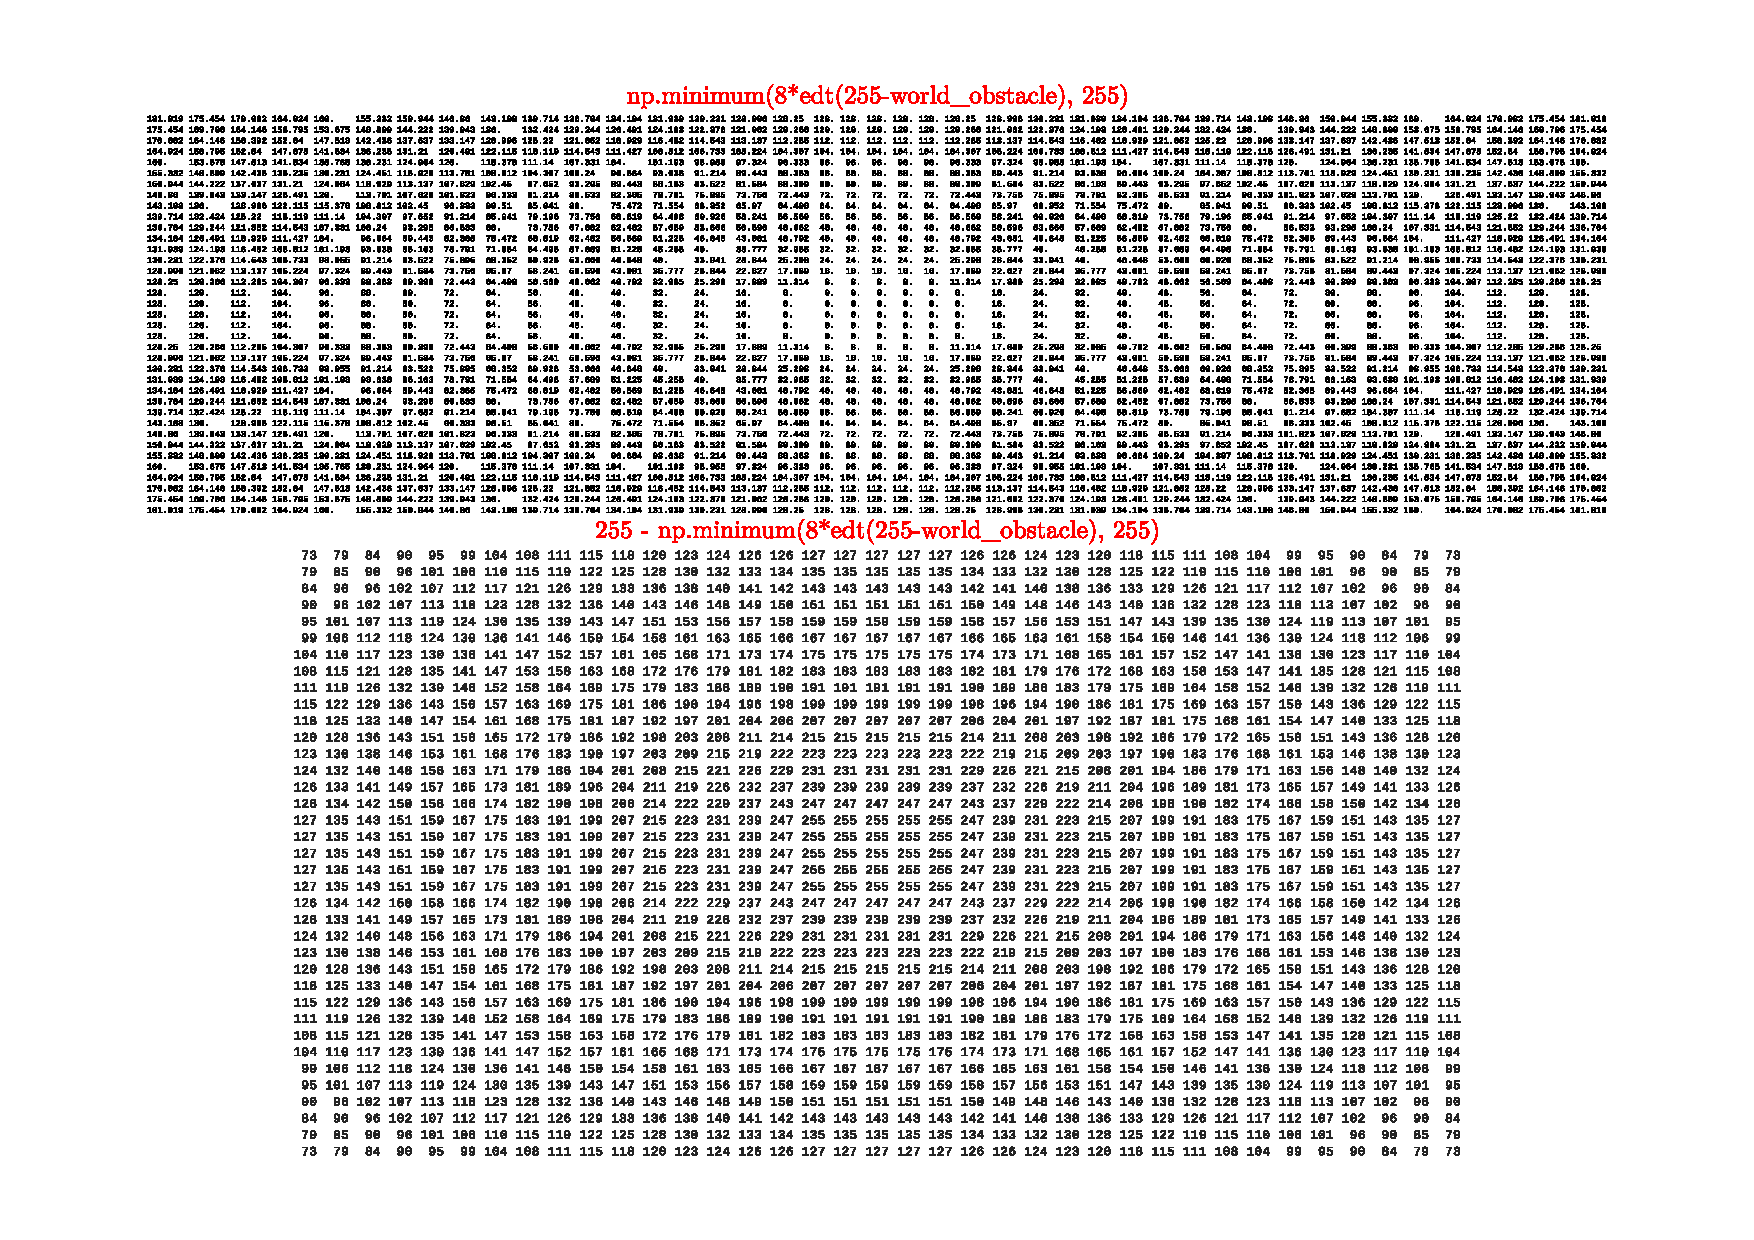
\includepdf[landscape=true]{../FIGURES/fig52.pdf}

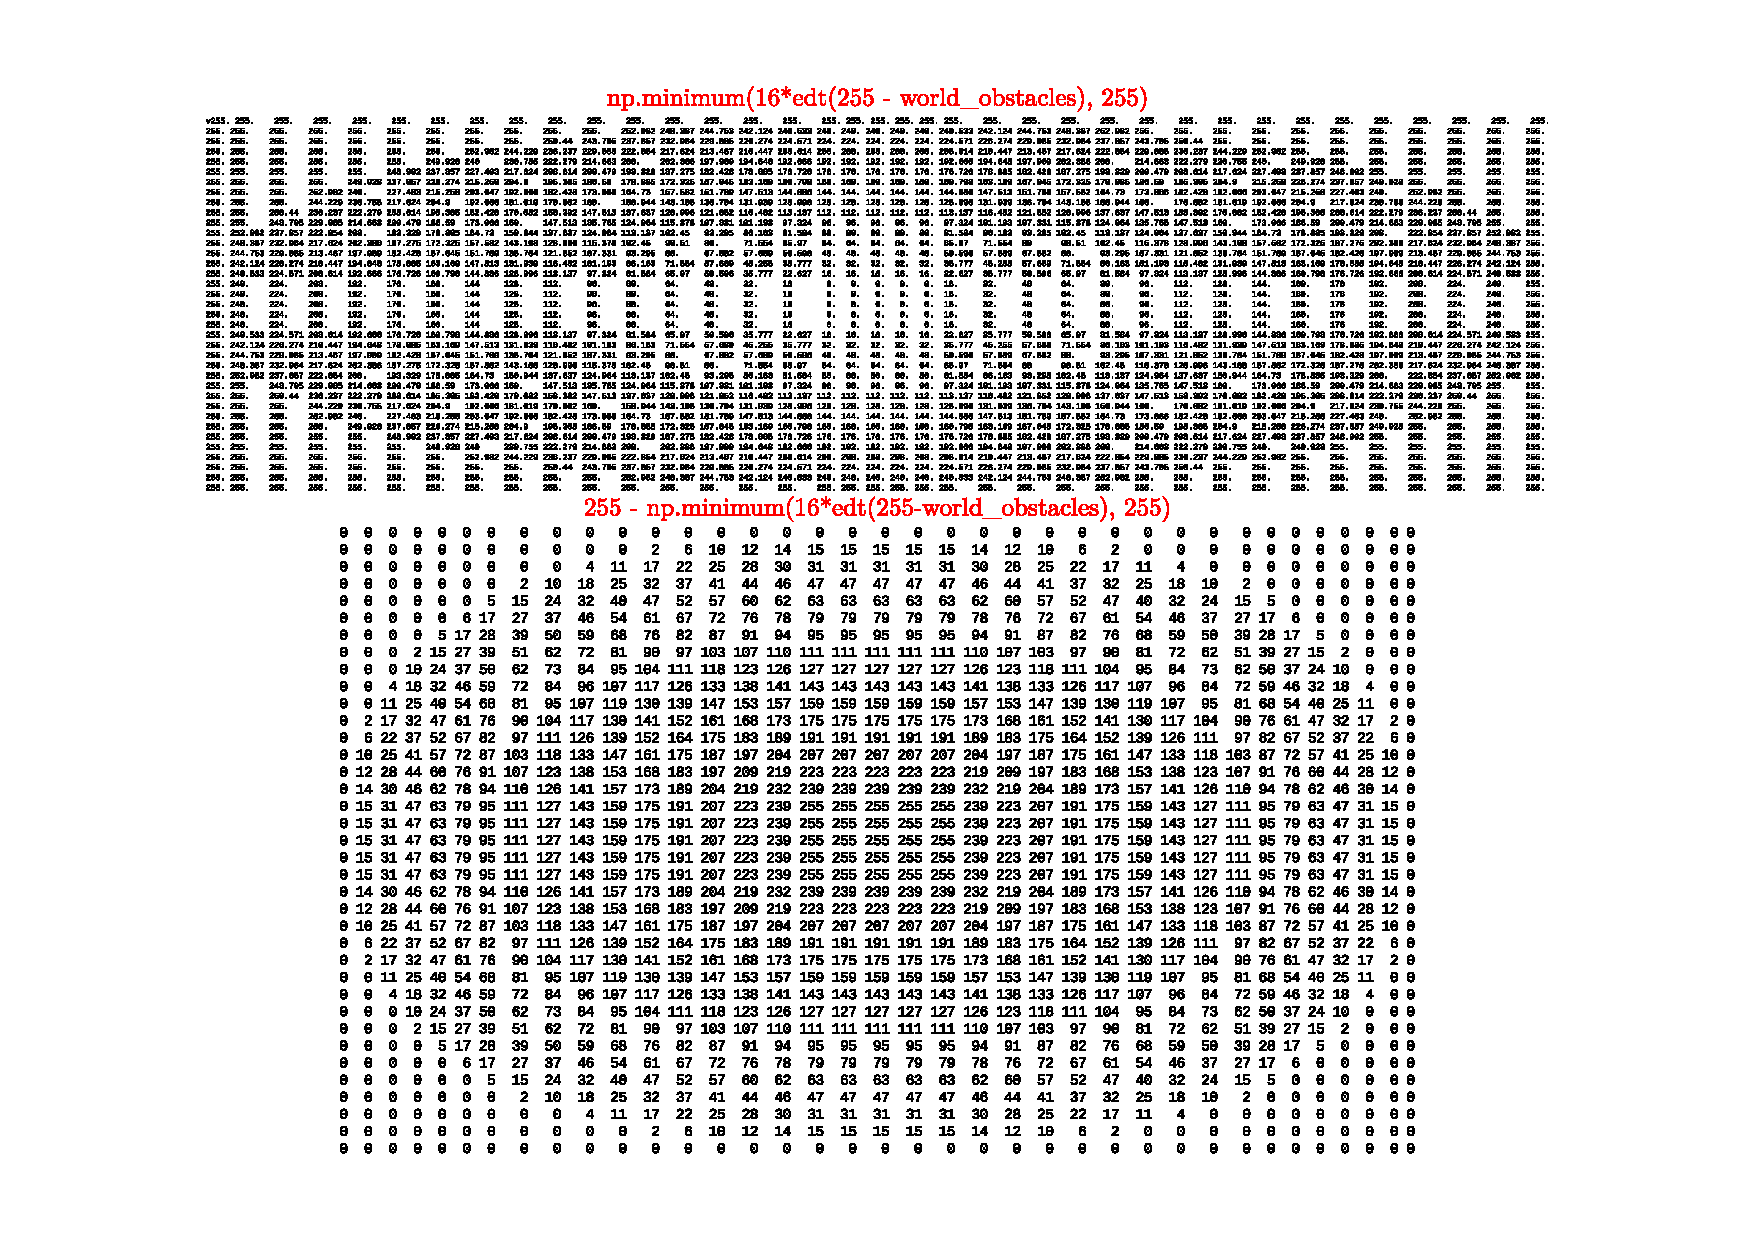
\includepdf[landscape=true]{../FIGURES/fig54.pdf}

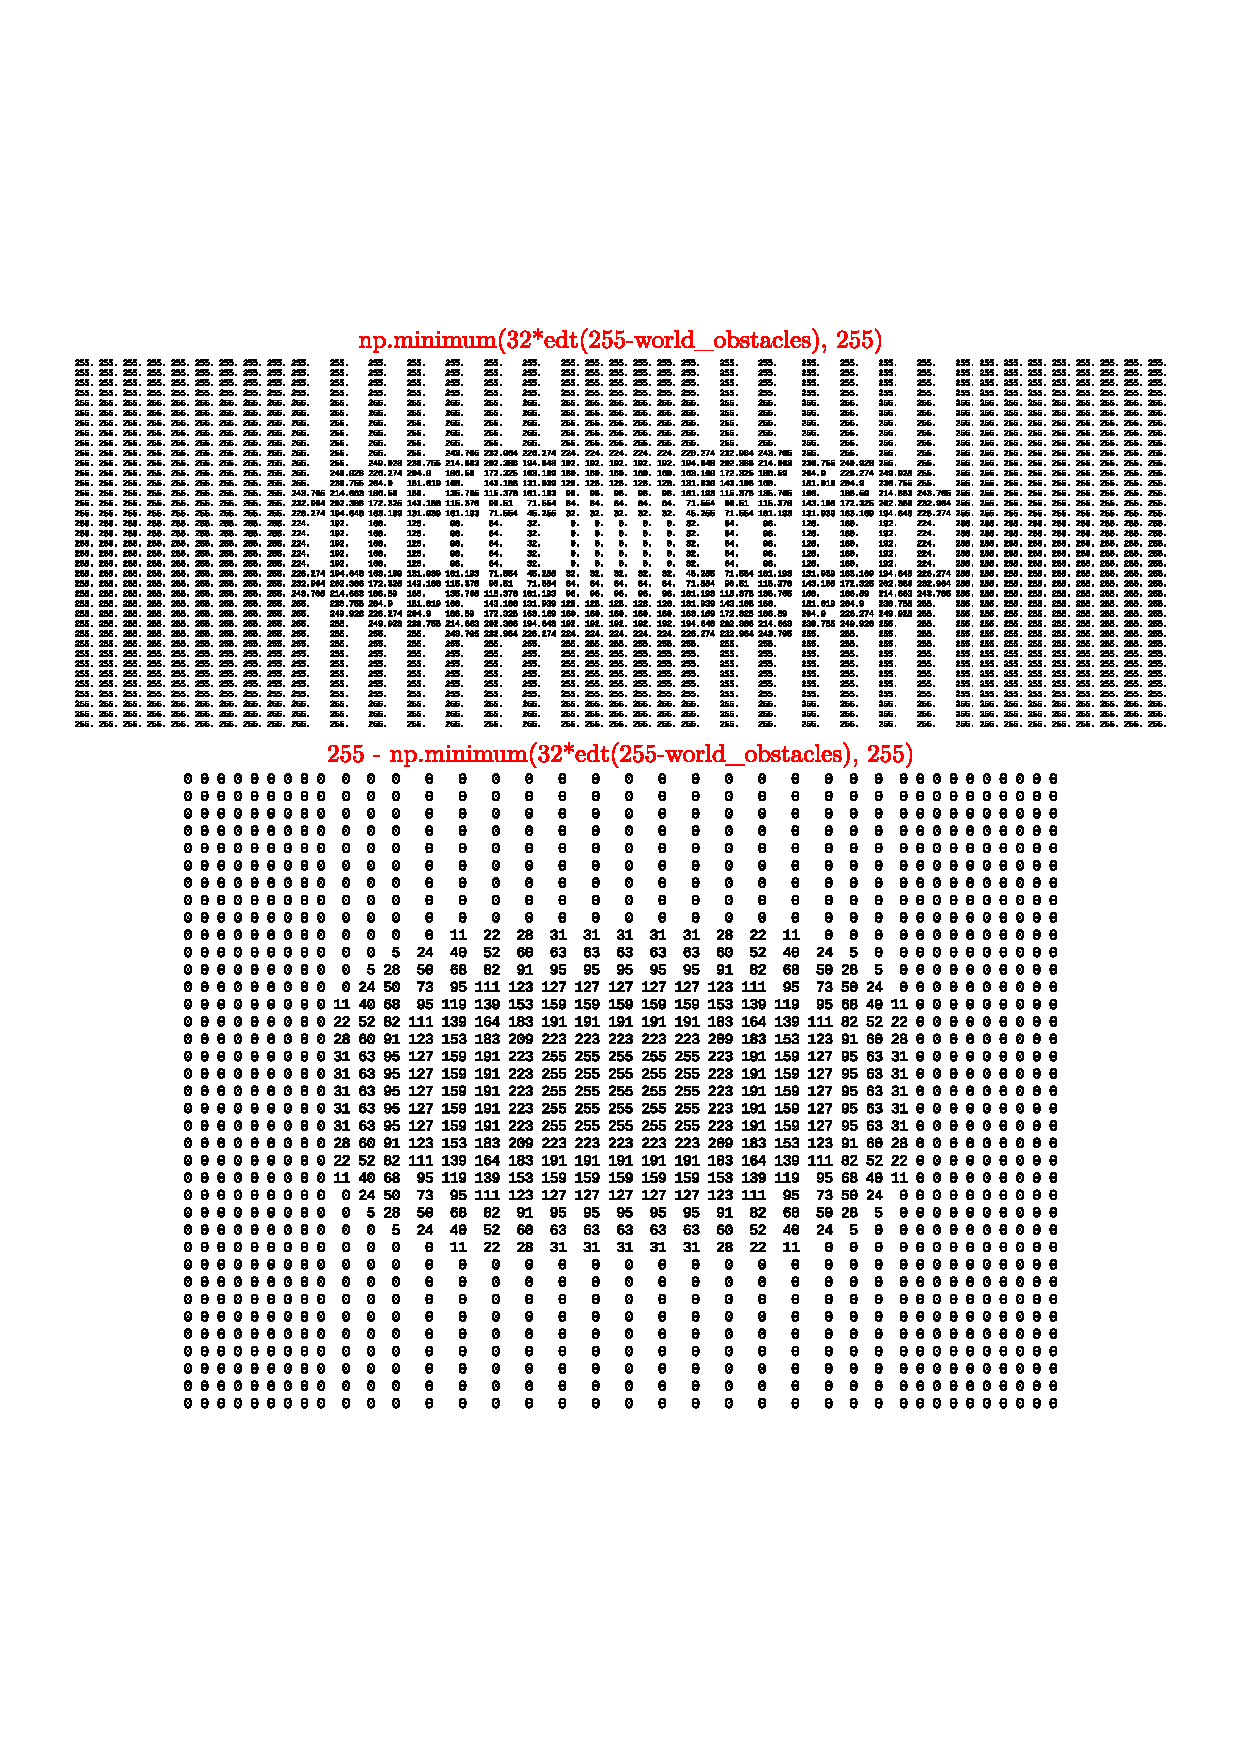
\includepdf{../FIGURES/fig56.pdf}

The cost associated to the node $world\_map \left( i, \, j \right)$
due to the presence of a potential field around the obstacles is:

\[
cost_{PF}(i\text{, j)=\ensuremath{\frac{{world\_map(i,j)}}{64}}}
\]

where $\left(i, j\right)$ are the i-th row and the j-th column in
the \texttt{world\_map} matrix. The above equation uses values of
the \texttt{world\_map} between 0 and 254.

Remember:
\begin{itemize}
\item The value $world\_map\left(i, \, j\right) \,= \, 0$, in these path
planning lectures, represents a free space node and any path can pass
through that node.
\item The value $world\_map\left(i, \, j\right) \,= \, 255$, in these path
planning lectures, represents an obstacle node and no one path can
pass through that node. This value can't be used in the above equation.
\end{itemize}
%
The total cost associated to the node $world\_map \left( i, \, j \right)$
is:

$total\_cost\left(i,\, j\right) \, = \, A \, + \, B \, + \, C \, + \, D$

where:
\begin{itemize}
\item A is the total cost of the previous node in the path.
\item B is the cost of the transition between the previous node in the path
and the current node ($world\_map \left( i, \, j \right)$).
\item C is the cost associated to the node $world\_map \left( i, \, j \right)$
due to the presence of a potential field around the obstacles, $cost_{PF} \left( i, \, j \right)$.
\item D is the estimated Euclidean distance between the current node ($world\_map \left( i, \, j \right)$)
and the goal node.
\end{itemize}
\begin{figure}[H]
\centering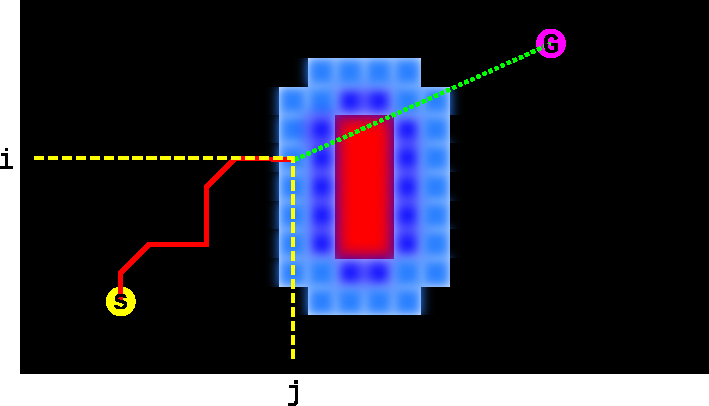
\includegraphics{../FIGURES/fig62}
\end{figure}

\begin{figure}[H]
\centering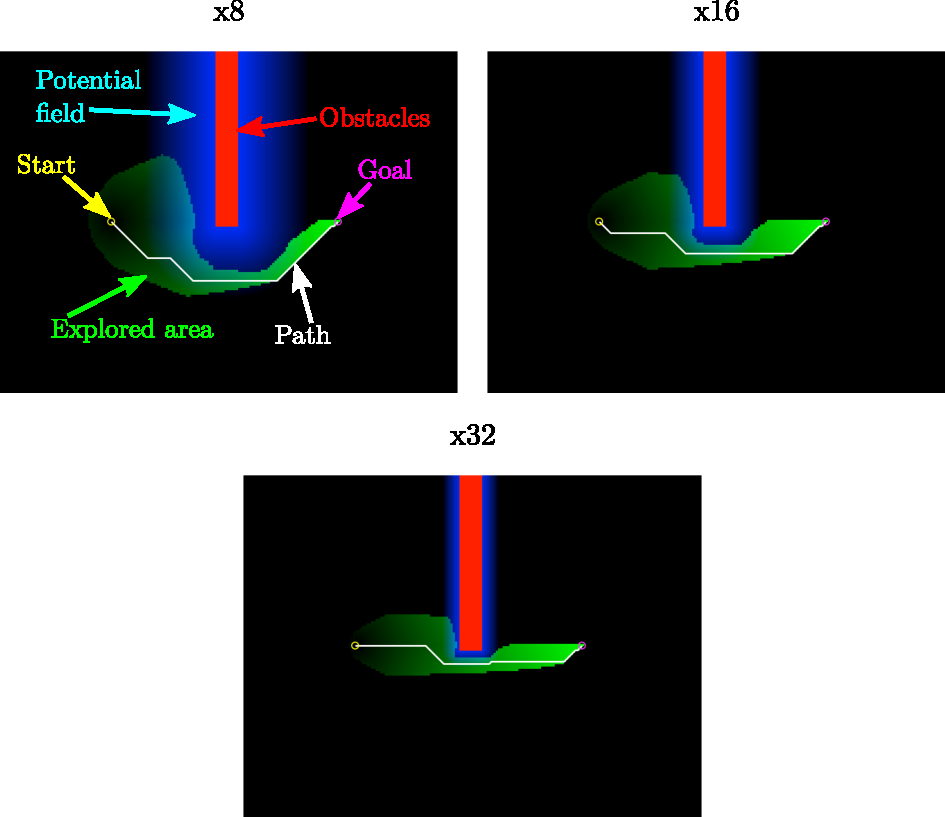
\includegraphics[scale=0.95]{../FIGURES/fig63}
\end{figure}

\end{document}
